\documentclass[12pt, a4paper]{article}
\usepackage[utf8]{inputenc}
\usepackage[brazilian]{babel} % Hifenização e dicionário
\usepackage[left=3.00cm, right=2.00cm, top=3.00cm, bottom=2.00cm]{geometry}
\usepackage{enumitem} % Para itemsep etc
\usepackage{longtable} % Dependência do longtabu
\usepackage{tabu} % Para melhor criação de tabelas
\usepackage{zi4} % Para fonte de códigos
\usepackage{listings} % Para códigos
\usepackage{lstautogobble} % Códigos indentados corretamente
\usepackage{color} % Para coloração de códigos
\usepackage{mathpazo} % Palatino
\usepackage{parskip} % Linha em branco entre parágrafos em vez de recuo
\usepackage{graphicx}
\usepackage{verbatim} % Para comentários
\usepackage{amsmath} % bmod
\usepackage[breaklinks]{hyperref}

\DeclareGraphicsExtensions{.pdf,.png}

\newcommand{\code}[1]{{\lstinline{#1}}}

\usepackage{listings}
\lstset{
    autogobble,
    columns=fullflexible,
    showspaces=false,
    showtabs=false,
    breaklines=true,
    showstringspaces=false,
    breakatwhitespace=true,
    escapeinside={(*@}{@*)},
    basicstyle=\ttfamily\footnotesize,
    frame=l,
    framesep=12pt,
    xleftmargin=12pt,
    tabsize=4,
    captionpos=b
}

\begin{document}
\begin{center}
    \textsc{Universidade Federal do Rio Grande do Norte} \\
    \textsc{Departamento de Informática e Matemática Aplicada}
\end{center}

\bigskip

\begin{tabular}{@{}ll@{}}
    \emph{Disciplina:} & DIM0612 --- Programação Concorrente \\
    \emph{Docente:}    & Everton Ranielly de Sousa Cavalcante \\
    \emph{Discente:}   & Felipe Cortez de Sá \\
\end{tabular}

\bigskip

\begin{center}
\large Multiplicação de matrizes
\end{center}

\bigskip

\section{Introdução}
Este relatório descreve a implementação de algoritmos para multiplicação de
matrizes de forma sequencial e usando múltiplas threads, detalhando as
estratégias utilizadas e comparando resultados.

\section{Detalhes da implementação}
O problema foi resolvido utilizando a linguagem de programação C++11 com a
biblioteca \code{std::thread}. No Mac foi selecionado o compilador \code{clang}
e em Ubuntu \code{g++}, ambos utilizando a flag \code{-O2} para otimizações. As
matrizes $ A $, $ B $ e $ C $ foram codificadas como vetores (arrays estilo C)
de tamanho $ n^2 $.

Na implementação com $ t $ \emph{threads}, cada thread é responsável pelo
cálculo de $ \frac{n^2}{t} $ elementos da matriz $ C $. Caso a divisão não seja
exata, a última thread calcula o resto, ou seja, $ \frac{n^2}{t} + (n^2 \mod t)
$ elementos. As threads são criadas pelo método \code{emplace\_back}, que
inicializa as threads da função \code{multThread} com os parâmetros que seguem.
% Reescreva essa frase pelo amor de deus

\begin{figure}[h]
\centering
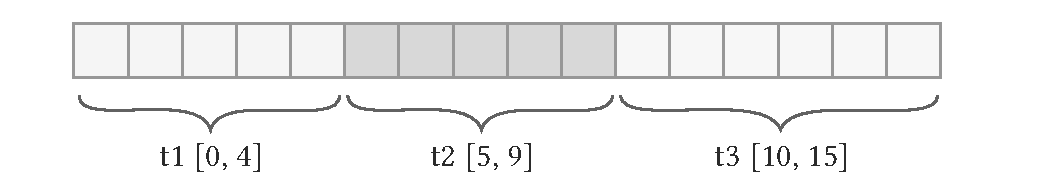
\includegraphics[width=.7\textwidth]{diagram_1}
\label{fig:f1}
\caption{Matriz $ C $ $ 4x4 $ com três threads}
\end{figure}

\subsection{Medição de desempenho}
Foi utilizada a biblioteca \code{std::chrono} para medir o tempo de execução.
Na implementação sequencial, o \emph{timer} inicia antes dos laços de
multiplicação e para depois dos laços. Na implementação com \emph{threads}, o
\emph{timer} inicia no momento anterior à criação da primeira \emph{thread} e o
posterior ao último \code{join()}.

\subsection{Testes}
Os testes foram automatizados com um script programado em \emph{Python} que
executa os programas sequencial e concorrente com valores diferentes para
número de threads utilizadas e retorna o mínimo, médio e máximo, bem como
desenha gráficos comparando as velocidades de execução para cada configuração.

\section{Resultados}
\begin{table}[h]\footnotesize
    \centering
    \begin{tabular}{ l | r r r }
        Caso      & mínimo & média & máximo \\
        \hline
        Sequencial & 2 & 3 & 4 \\
        2 threads  & 5 & 6 & 4 \\
        3 threads  & 8 & 9 & 4 \\
        4 threads  & 8 & 9 & 4 \\
    \end{tabular}
  \caption{Para n = .22l2l2}
\end{table}

\section{Discussão}
A partir da realização desse trabalho foi possível concluir que o uso de
threads pode aumentar o desempenho na resolução de problemas paralelos.

\end{document}
